\documentclass[a4paper, 10pt, titlepage]{article}

\usepackage{inputenc,enumitem,graphicx,caption,float,amsmath,bbold,mathtools}
\usepackage[svgnames]{xcolor}
\usepackage{listings}
\usepackage[left=2.5cm, right=4cm, top=2cm]{geometry}
\usepackage{makecell}
\usepackage[section]{placeins}
\makeatletter
\AtBeginDocument{%
  \expandafter\renewcommand\expandafter\subsection\expandafter{%
    \expandafter\@fb@secFB\subsection
  }%
}
\makeatother
\newcommand*\rot{\rotatebox{90}}
\newcommand\Tstrut{\rule{0pt}{2.9ex}}         % "top" strut
\newcommand\Bstrut{\rule[-1.2ex]{0pt}{0pt}}   % "bottom" strut
\newcommand\TBstrut{\Tstrut\Bstrut}           % "top and bottom" strut
\makeatletter
\def\verbatim{\small\@verbatim \frenchspacing\@vobeyspaces \@xverbatim}
\makeatother
\lstset{language=R,
    basicstyle=\small\ttfamily,
    stringstyle=\color{DarkGreen},
    otherkeywords={0,1,2,3,4,5,6,7,8,9},
    morekeywords={TRUE,FALSE},
    deletekeywords={data,frame,length,as,character},
    keywordstyle=\color{blue},
    commentstyle=\color{DarkGreen},
}

% \usepackage[english]{babel}
% \usepackage[utf8]{inputenc}
% \usepackage{amsmath,amsfonts}
% \usepackage{mathtools}
% \usepackage{graphicx}
% \usepackage{graphics}
% \usepackage[colorinlistoftodos]{todonotes}
% \usepackage[margin=1in]{geometry}
% \usepackage{enumitem}
% \usepackage{caption}
% \usepackage{multirow}
% \usepackage{fancyvrb}
% \usepackage{xcolor}
% \usepackage{float,bbold}
% \captionsetup[table]{skip=10pt}
% \newcommand*\rot{\rotatebox{90}}
% \usepackage[svgnames]{xcolor}
% \def\verbatim{\small\@verbatim \frenchspacing\@vobeyspaces \@xverbatim}
% \makeatother
% \lstset{language=R,
%     basicstyle=\small\ttfamily,
%     stringstyle=\color{DarkGreen},
%     otherkeywords={0,1,2,3,4,5,6,7,8,9},
%     morekeywords={TRUE,FALSE},
%     deletekeywords={data,frame,length,as,character},
%     keywordstyle=\color{blue},
%     commentstyle=\color{DarkGreen},
% }

\title{Effect of Air Movement on\\Chick Body Temperature}

\author{
        Elliot Outland \\
        Minjiao Yang
        }

\date{Prepared for Dr. Brian Fairchild on December 13\textsuperscript{th}, 2019 \\ 
        in Dr. Jaxk Reeves' STAT 8001 Course}

\begin{document}
\maketitle
\tableofcontents
\listoffigures
\listoftables

\newpage

\section*{Summary}
The purpose of this study was to provide a better understanding of aspects of chick breeding concerning temperature management. The data used in this analysis was collected from an experiment conducted on 2 repetitions of 3 brooding room temperature trials, consisting of 16 chicks each having their body temperature measured 5 times, twice a day over 7 days. Both rectal and flank temperature measurements were taken from the chicks and recorded. Using this data, we fit mixed models describing the relationship between flank and rectal body temperature, as well as the effect of exposing chicks to a fan blowing air at 200 ft/sec. We find that the rectal temperature can be reasonably accurately determined from flank temperature by subtracting a constant 0.1 on average, and that the precise effect of exposure to a fan varies with the ambient temperature; in an 85$^{\circ}$F brooding room, the chicks exposed to air movement had lower rectal and flank body temperatures by around 0.22$^{\circ}$C, chicks in a 90$^{\circ}$F brooding room showed evidence of approximately 0.32$^{\circ}$C lower rectal temperatures and 0.35$^{\circ}$C lower flank temperatures when exposed to the fan, and chicks in a 95$^{\circ}$F brooding room showed weak or insignificant evidence of lower rectal temperatures by 0.11$^{\circ}$C to 0.13$^{\circ}$C under exposure to the fan.

\section{Introduction}
Poultry represents a significant dietary and economic force in the United States, particularly in Georgia; Americans consumed approximately 107 lbs of chicken in 2017, and poultry represents 46\% of Georgia's agricultural economy, which itself represented \$4B of Georgia's GDP in 2017. Given the crucial role of poultry, it is of clear benefit to investigate means to improve poultry production. One area of particular concern to chicken breeders and researchers is chick temperature; temperatures that are too cold can lead to lethargic and weak chicks. In an effort to improve standard practices in chick temperature management, Dr. Fairchild's study seeks to answer the following questions:
\begin{enumerate}[label = (\alph*)]
	\item
		What is the relationship between rectal and flank temperature? Is flank temperature a suitable substitute for rectal temperature?
	\item
		How does exposure to air movement affect chick body temperatures?
\end{enumerate}

\section{Data Summary}
The data was collected from a set of experiments which were each conducted as follows:  16 one-day-old chicks were separated into control and treatment groups, each made up of 8 chicks. The body temperatures of the chicks in each group were measured rectally as well as through a chip embedded in the chicks’ flanks, with the rectal and flank temperatures each being recorded as separate observations. The chicks’ temperatures were measured in this fashion twice in a holding pen before the chicks were moved into individual treatment cells, where their temperatures were measured 3 more times in the same manner. In the cell period, the chicks in the treatment group were exposed to a fan blowing air at 200 ft/sec, while the chicks in the control group were not subjected to any air movement. This process was repeated twice per day, once in the morning and once in the afternoon, for 7 days (days one through seven of the chicks' lives). The experiment was conducted under 3 brooding temperatures (85$^{\circ}$F, 90$^{\circ}$F, and 95$^{\circ}$F), with the trials under each temperature each using a different set of 16 chicks. The researchers conducted 2 repetitions of the experiment at each brooding temperature. Taken together, these factors give a total of 13,440 (= 3 brooding temperatures $\times$ 2 reps $\times$ 2 conditions $\times$ 8 chicks $\times$ 7 days $\times$ 2 times-of-day $\times$ 5 measurements $\times$ 2 measurement locations) observations; however, 80 of the observations under the 85$^{\circ}$ were missing, instead giving a total of 13,360 observations (or 6,680 (rectal, flank) pairs of measurements). The variables present in the original data-set are summarized in Table~\ref{table:original air data}.

\begin{table}[ht]
	\centering
	\captionof{table}{Original air movement data summary.}
	\begin{tabular}{|l|l|l|}
		\hline
		\textbf{Variable} & \textbf{Type} & \textbf{Levels}\\
		\hline
		Room Temp & Factor & 85, 90, 85\\
		Rep & Factor & 1, 2\\
		Day & Factor & 1, 2, 3, 4, 5, 6, 7\\
		Time of Day & Date-Time & \\
		Period & Factor & P, T\\
		Location & Factor & R, W\\
		Group & Factor & Ctrl, Trt\\
		Sensor Number & Factor & 19 distinct sensors\\
		Air Velocity & Factor & 0, 200 ft/sec\\
		Age & Continuous & \\
		Body Temp & Continuous & \\
		Set & Factor & 1, 2, 3\\
		Trial & Factor & 1, 2, 3\\
		Parent Flock Age & Factor & 37, 40, 44, 46, 47, 60\\
		Period + Set & Factor & P1, P2, P3, T1, T2, T3\\
		\hline
		\multicolumn{3}{|c|}{13,360 observations}\\
		\hline
	\end{tabular}
	\label{table:original air data}
\end{table}
\par
Before conducting our analyses, we identified 5 variables (`Air Velocity', `Set', `Trial', `Parent Flock Age', and `Period + Set') which proved to be either redundant or of little value, and were thus discarded. The variables that were retained were re-coded, and an additional variable identifying individual chicks was added. Finally, we averaged the 2 pen and 3 holding cell temperatures during each time of measurement (i.e., morning and afternoon), resulting in 4 body temperature measurements per chick per time of day; using the mean values allowed us to obtain one-to-one occurrences of pen and cell body temperature measurements for each chick. The transformed data is given in Table~\ref{table:transformed air data}. 

\begin{table}[ht]
	\centering
	\captionof{table}{Transformed air movement data summary.}
	\begin{tabular}{|l|l|l|}
		\hline
		\textbf{Variable} & \textbf{Type} & \textbf{Levels}\\
		\hline
		Room Temp & Factor & 0 (85), 1 (90), 2 (85)\\
		Rep & Factor & 1, 2\\
		Day & Factor & 1, 2, 3, 4, 5, 6, 7\\
		Time of Day & Factor & 0 (AM), 1 (PM)\\
		Location & Factor & 0 (Rectal), 1 (Flank)\\
		Group & Factor & 0 (Ctrl), 1 (Trt)\\
		Chick Id & Factor & 96 distinct chicks\\
		Pen Body Temp & Continuous & \\
		Cell Body Temp & Continuous & \\
		\hline
		\multicolumn{3}{|c|}{2,672 observations}\\
		\hline
	\end{tabular}
	\label{table:transformed air data}
\end{table}

\section{Exploratory Data Analysis}
\subsection{EDA for Flank vs. Rectal Investigation}
We begin our investigation into the relationship between flank and rectal temperature by plotting them against one another in Figure~\ref{figure:rectal wing plt}.

\begin{figure}[]
	\centering
		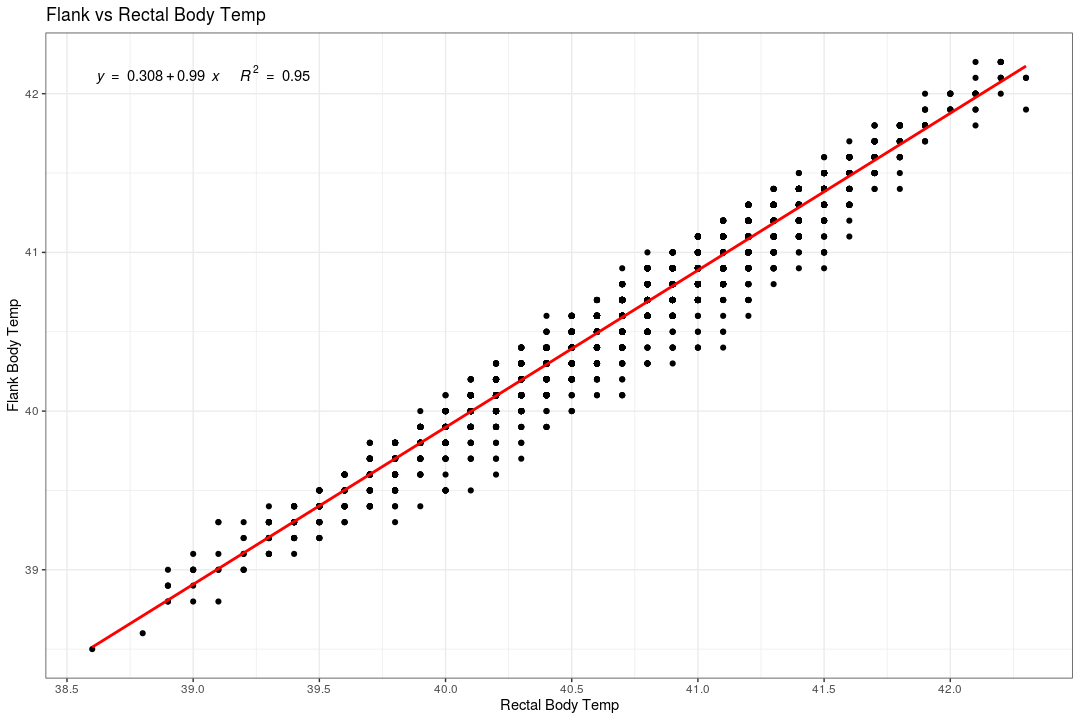
\includegraphics[width = 0.75\textwidth]{images/rectal_wing_plt.png}
	\caption{Plot of rectal vs flank temperature with regression line.}
	\label{figure:rectal wing plt}
\end{figure}

Note the consistent spacing between the points; the temperature sensor used to conduct the experiment outputs measurements in units of 0.1${^\circ}$C, so the points in the figure are discrete to that level of precision. The linear relationship between rectal and flank temperatures can easily be observed by visual inspection, and a regression line can be drawn through the points. 

However, upon examining the residual values plotted in Figure~\ref{figure:rectal wing res}, we see that they tend to skew negative. 

\begin{figure}[]
	\centering
		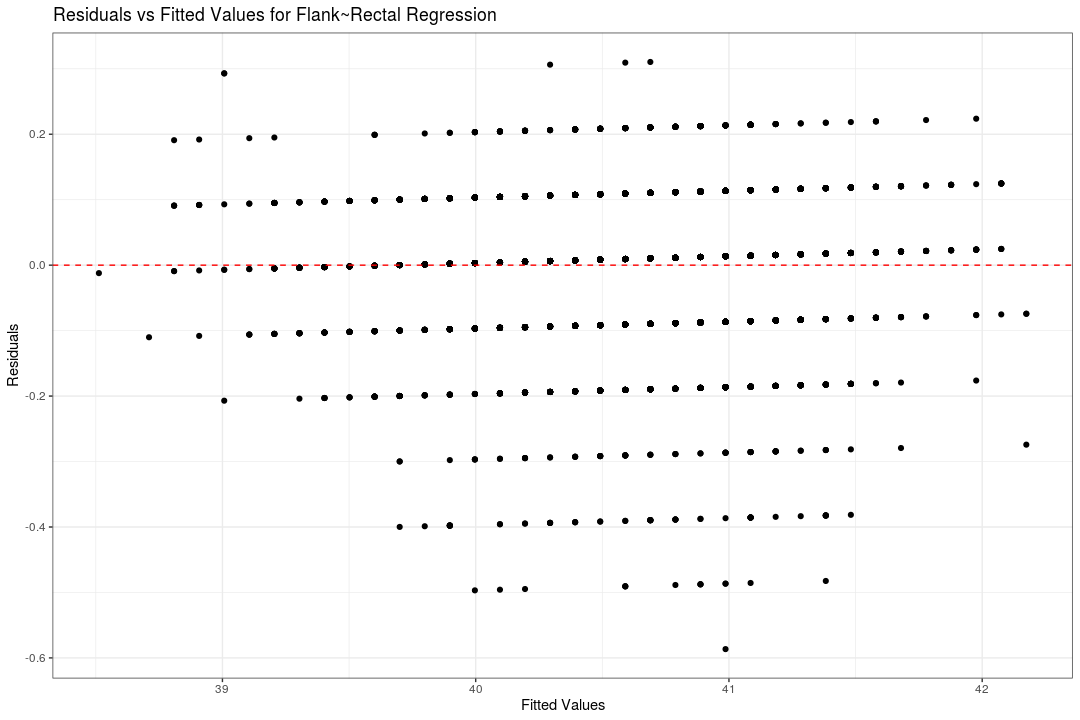
\includegraphics[width = 0.75\textwidth]{images/flank_rectal_residuals.png}
	\caption{Plot of residuals for rectal vs flank regression.}
	\label{figure:rectal wing res}
\end{figure}

Drawing a histogram for the distribution of the difference between flank and rectal temperature ($\textrm{Diff} = \textrm{Flank} - \textrm{Rectal}$) provides further evidence of outliers that might skew the data; this can be seen in Figure~\ref{figure:rectal wing hist}.

\begin{figure}[]
	\centering
		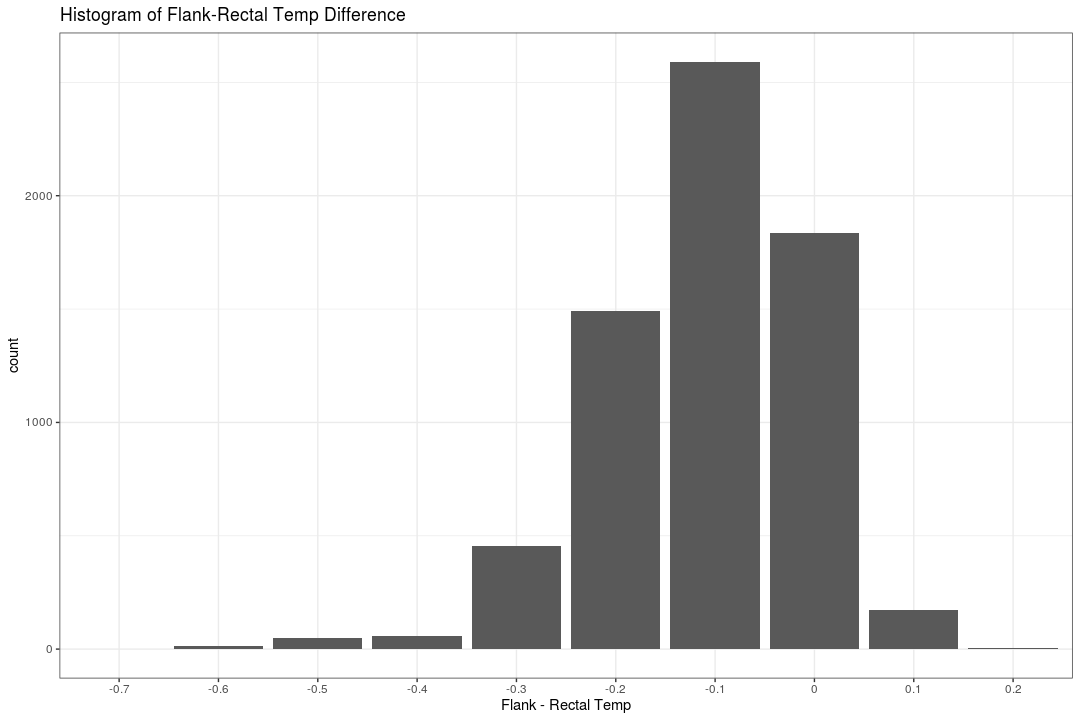
\includegraphics[width = 0.75\textwidth]{images/flank_rectal_hist.png}
	\caption{Histogram of $\textrm{Flank} - \textrm{Rectal}$ difference in temperature measurements.}
	\label{figure:rectal wing hist}
\end{figure}

\subsection{EDA for Cell Body Temperature Analyses}
The box plots in Figure~\ref{figure:factor boxplots} provide some clues as to the nature of the relationships between chick body temperature and the various factors that might influence it. We see immediately that the treatment group has a lower mean temperature than the control group, which could indicate that exposure to a fan tends to lower the temperature of chicks. The time-of-day plot seems to suggest that chick temperatures vary less in the afternoon than in the morning, since the boxes are more compact. We also see indication that warmer brooding rooms tend to have warmer chicks. The box plots for the age factor display the known fact that chicks tend to become better at regulating body temperature as they grow older. Finally, the plot for experimental repetition shows mild evidence of between-rep variability in temperature measurements.

\begin{figure}[!h]
	\centering
		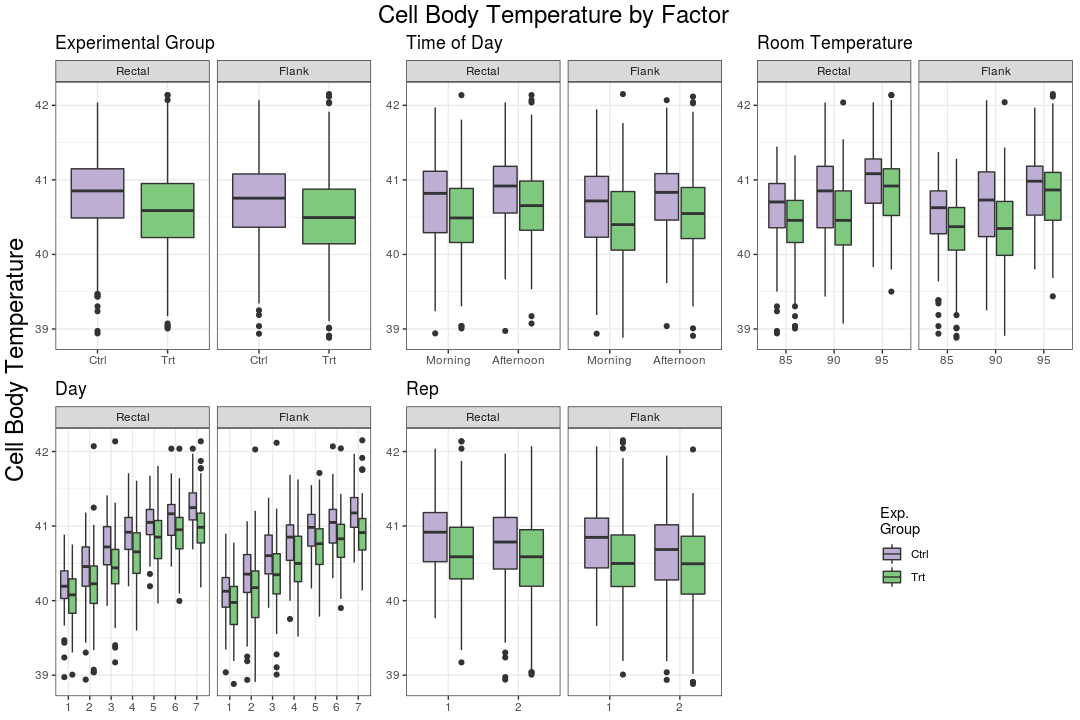
\includegraphics[width = 0.75\textwidth]{images/boxplots.png}
	\caption{Box plots of cell temperature by possible explanatory factors.}
	\label{figure:factor boxplots}
\end{figure}

\section{Analysis}
The trends that we have observed during our exploratory data analysis provide us with a framework under which to conduct our analysis.

\subsection{Relationship Between Flank and Rectal Body Temperature}
	We begin our statistical analysis by examining the relationship between flank and rectal temperature. This analysis was conducted on the non-transformed data-set, since each rectal body temperature measurement could be paired with a corresponding flank temperature measurement without the need for averaging.
	
\par

    As we saw in Figure~\ref{figure:rectal wing hist} during our exploratory analysis, the distribution of the \textit{difference} in flank and rectal temperature has several outliers that may obfuscate the true relationship between readings from the two measurement locations. We address this by excluding values falling outside of the interval $[-0.3, 0.1]$, which contains approximately 98\% of the observations. After removing the outliers, we first fit a model for Flank incorporating main effects for `Rep', `Day', `Time of Day', `Group', the two-way interactions between them, and a random chick effect. The interaction effects and all main effects aside from 'Day' were found to be insignificant and so were dropped from the model.
    
\par

    Our final model thus follows:
	
\begin{align}
y_{ijkl} = \mu + \alpha_h + b_{jkl} + \epsilon_{ijkl},
\end{align}
{\renewcommand{\arraystretch}{1.5}
\begin{tabular}{ll}
     where  & $y_{ijkl}$ is the Flank-Rectal body temperature \textit{difference}\\
            & $\mu$ is the grand mean\\
            & $\alpha_i$ is the $i^{th}$ day effect, with $i = 1,\dots,7$\\
            & \makecell[l]{$b_{jkl}$ is the random effect for the, $l^{th}$ chick under the $k^{th}$ temperature trial in the \\ $j^{th}$ rep, with $l = 1,\ldots,16$, $k = 0, 1, 2$, and $j = 1, 2$}\\
            & $\epsilon_{ijkl}$ is random error.
\end{tabular}\\}

The above model is similar to the familiar ANOVA model in that it estimates the significance of the difference in means across a given factor (in this case `Day'); however, the addition of a random effect (the `chick' effect) allows us to account for individual variation between chicks. This is relevant to our case since the experiment under analysis relies on repeated measurements of the same chicks within a brooding temperature trial.

    The estimates for this model are given in Table~\ref{table:Est FR rel}, with the ANOVA tables available in the appendix.
    
\begin{table}[ht]
\centering
\captionof{table}{Estimates for explanatory variables affecting Flank-Rectal temperature difference.} 
\begin{tabular}[t]{lrr}
 \hline
 \multicolumn{3}{c}{\textbf{Fixed Effects}}\\
 \hline
 & \textbf{Estimate} & \textbf{p-value}\Tstrut\\ 
 Intercept & -0.1024 & $<$0.0001\\
 Day 2 & -0.0061 & 0.0744\\
 Day 3 & -0.0115 & 0.0007\\
 Day 4 & -0.0125 & 0.0003\\
 Day 5 & -0.0006 & 0.8679\\
 Day 6 & -0.0044 & 0.2045\\
 Day 7 & 0.0126 & 0.0002\\
 \hline
\end{tabular}
\quad
\begin{tabular}[t]{lrr}
 \hline
\multicolumn{3}{c}{\textbf{Random Effect}}\\
 \hline
 & \textbf{Chick} & \textbf{Residual}\Tstrut \\ 
 Std Dev & 0.0608 & 0.0741\Bstrut\\
 \hline
\end{tabular}
\label{table:Est FR rel}
\end{table}

Note that the above model uses `Day 1' as a baseline. The intercept value of -0.1024 then suggests that the expected Flank-Rectal difference in a day-old chick is -0.1024, while the difference for a two-day-old chick is expected to be $-0.1024 - 0.0061 = -0.1085$, and the expected difference for a three-day-old chick is $-0.1024 - 0.0115 = -0.1139$; the values for older chicks can be calculated similarly. This difference varies somewhat as the chick grows older, but averages to -0.1056 across all days, with a between-chick variation of 0.0608 degrees, and a typical unexplained error (after accounting for other fixed and random effects), with a mean of zero and standard deviation of 0.0741. 

\subsection{Effect of Air Movement on Chick Body Temperature}
We now address the issue of explaining the effect of air movement on chicks’ body temperatures. We adopt an approach similar to that which we used in answering the first question, fitting a linear model with random effects accounting for the individual variation between the chicks in each replication of the experiment. Since it is feasible that the effect of air movement might vary across brooding room temperatures, we elected to build separate models for each of the 85$^{\circ}$F, 90$^{\circ}$F, and 95$^{\circ}$F brooding room temperatures for both flank and rectal temperatures. For each of the aforementioned 6 cases, we first fit the full model with `Cell Body Temperature' as the response, and the main effects `Time of Day', `Day', `Rep', and `Group', as well as the interaction effects between them, a random chick effect, and a co-variate representing `Pen Body Temperature' as the explanatory model. After fitting the model to the data, we found the interaction terms to be insignificant, and so dropped them from the model. We also eliminated the co-variate; since both the random effect and co-variate both capture, in some sense, the individual variation in chicks, inclusion of both was deemed unnecessary. Also contributing to this decision was the practical concern that it would be undesirable for a party who is only interested in estimating a given chick's body temperature under a fan to be required to first obtain the chick's temperature in a holding pen. 

\par 

After making the adjustments outlined above, we arrive at the model given in Equation (2), which was fit for each of the 6 (location, temperature) pairs:

\begin{align}
	y_{hijkl} = \mu + \alpha_h  + \beta_i + \gamma_j + \tau_k + b_{hl} + \epsilon_{hijkl},
\end{align}
{\renewcommand{\arraystretch}{1.5}
\begin{tabular}{ll}
     where  & $y_{hijkl}$ is the averaged cell rectal/flank body temperature at 85$^{\circ}$\textbackslash95$^{\circ}$\textbackslash95$^{\circ}$\\
            & $\mu$ is the grand mean\\
            & $\alpha_h$ is the $h^{th}$ rep effect, with $h = 1, 2$\\
            & $\beta_i$ is the $i^{th}$ day effect, with $i = 1,\ldots,7$\\
            & $\gamma_j$ is the $j^{th}$ time-of-day effect, with $j = 0, 1$ (0 = morning, 1 = afternoon)\\
            & $\tau_k$ is the $k^{th}$ group effect, with $k = 0, 1$ (0 = control, 1 = treatment)\\
            & $b_{hl}$ the random effect for the $l^{th}$ chick in the $h^{th}$ rep, with $l = 1,\ldots,16$\\
            & $\epsilon_{hijkl}$ is random error.
\end{tabular}\\}

Estimates for the above model are given in the tables below; ANOVA tables are presented in the appendix:

\begin{table}[ht]
\centering
\captionof{table}{Estimates for explanatory variables for \textit{rectal} body temperature under \textit{85$^{\circ}$} brooding temperature.} 
\begin{tabular}[t]{lrr}
 \hline
 \multicolumn{3}{c}{\textbf{Fixed Effects}}\\
 \hline
 & \textbf{Estimate} & \textbf{p-value}\Tstrut\\ 
 Intercept & 40.0969 & $<$0.0001\\
 2$^{nd}$ Rep & -0.0463 & 0.4533\\
 Day 2 & 0.1920 & 0.0002\\
 Day 3 & 0.3954 & $<$0.0001\\
 Day 4 & 0.5668 & $<$0.0001\\
 Day 5 & 0.7422 & $<$0.0001\\
 Day 6 & 0.8144 & $<$0.0001\\
 Day 7 & 0.9075 & $<$0.0001\\
 \textbf{Treatment} & \textbf{-0.2182} & \textbf{0.0012}\\
 \makecell[l]{Time of Day \\ (PM)\Bstrut} & 0.0758 & 0.0067\\
 \hline
\end{tabular}
\quad
\begin{tabular}[t]{lrr}
 \hline
\multicolumn{3}{c}{\textbf{Random Effect}}\\
 \hline
 & \textbf{Chick} & \textbf{Residual}\Tstrut \\ 
 Std Dev & 0.1528 & 0.2914\Bstrut\\
 \hline
\end{tabular}
\label{table:Est 85 R}
\end{table}

\begin{table}[ht]
\centering
\captionof{table}{Estimates for explanatory variables for \textit{flank} body temperature under \textit{85$^{\circ}$} brooding temperature.} 
\begin{tabular}[t]{lrr}
 \hline
 \multicolumn{3}{c}{\textbf{Fixed Effects}}\\
 \hline
 & \textbf{Estimate} & \textbf{p-value}\Tstrut\\ 
 Intercept & 40.0476 & $<$0.0001\\
 2$^{nd}$ Rep & -0.0701 & 0.2229\\
 Day 2 & 0.1638 & 0.0016\\
 Day 3 & 0.3540 & $<$0.0001\\
 Day 4 & 0.5339 & $<$0.0001\\
 Day 5 & 0.7148 & $<$0.0001\\
 Day 6 & 0.7867 & $<$0.0001\\
 Day 7 & 0.8802 & $<$0.0001\\
 \textbf{Treatment} & \textbf{-0.2201} & \textbf{0.0005}\\
 \makecell[l]{Time of Day \\ (PM)\Bstrut} & 0.0708 & 0.0114\\
 \hline
\end{tabular}
\quad
\begin{tabular}[t]{lrr}
 \hline
\multicolumn{3}{c}{\textbf{Random Effect}}\\
 \hline
 & \textbf{Chick} & \textbf{Residual}\Tstrut \\ 
 Std Dev & 0.1379 & 0.2923\Bstrut\\
 \hline
\end{tabular}
\label{table:Est 85 F}
\end{table}

For the 85$^{\circ}$F trial, we can see that both the rectal and flank temperatures of the chicks in the treatment group  are significantly lower than those in the control group by about 0.22$^{\circ}$C. There also appears to be a significant age effect on chicks’ body temperatures; as the days increase, the chicks' body temperatures increase, which mirrors what we saw during our exploratory analysis. The temperatures increase rapidly until day 5, where they become more stable. In addition, the time-of-day estimate suggests that the chicks’ rectal and flank temperatures are higher in the afternoon than in the morning. It may be the case that chicks’ body temperatures are higher in the afternoon since the afternoon is generally warmer. The random effect has a non-zero standard deviation, suggesting the presence of a between-chick variation of around 0.14$^{\circ}$C to 0.15$^{\circ}$C.

\begin{table}[ht]
\centering
\captionof{table}{Estimates for explanatory variables for \textit{rectal} body temperature under \textit{90$^{\circ}$} brooding temperature.} 
\begin{tabular}[t]{lrr}
 \hline
 \multicolumn{3}{c}{\textbf{Fixed Effects}}\\
 \hline
 & \textbf{Estimate} & \textbf{p-value}\Tstrut\\ 
 Intercept & 40.1664 & $<$0.0001\\
 2$^{nd}$ Rep & -0.1848 & 0.0038\\
 Day 2 & 0.1229 & 0.0083\\
 Day 3 & 0.4515 & $<$0.0001\\
 Day 4 & 0.6992 & $<$0.0001\\
 Day 5 & 0.8672 & $<$0.0001\\
 Day 6 & 0.9504 & $<$0.0001\\
 Day 7 & 1.1007 & $<$0.0001\\
 \textbf{Treatment} & \textbf{-0.3236} & \textbf{$<$0.0001}\\
 \makecell[l]{Time of Day \\ (PM)\Bstrut} & 0.2239 & $<$0.0001\\
 \hline
\end{tabular}
\quad
\begin{tabular}[t]{lrr}
 \hline
\multicolumn{3}{c}{\textbf{Random Effect}}\\
 \hline
 & \textbf{Chick} & \textbf{Residual}\Tstrut \\ 
 Std Dev & 0.1511 & 0.2602\Bstrut\\
 \hline
\end{tabular}
\label{table:Est 90 R}
\end{table}

\begin{table}[ht]
\centering
\captionof{table}{Estimates for explanatory variables for \textit{flank} body temperature under \textit{90$^{\circ}$} brooding temperature.} 
\begin{tabular}[t]{lrr}
 \hline
 \multicolumn{3}{c}{\textbf{Fixed Effects}}\\
 \hline
 & \textbf{Estimate} & \textbf{p-value}\Tstrut\\ 
 Intercept & 40.0709 & $<$0.0001\\
 2$^{nd}$ Rep & -0.2310 & 0.0037\\
 Day 2 & 0.1191 & 0.0108\\
 Day 3 & 0.4746 & $<$0.0001\\
 Day 4 & 0.6888 & $<$0.0001\\
 Day 5 & 0.8863 & $<$0.0001\\
 Day 6 & 0.9731 & $<$0.0001\\
 Day 7 & 1.1544 & $<$0.0001\\
 \textbf{Treatment} & \textbf{-0.3483} & \textbf{0.0001}\\
 \makecell[l]{Time of Day \\ (PM)\Bstrut} & 0.2264 & $<$0.0001\\
 \hline
\end{tabular}
\quad
\begin{tabular}[t]{lrr}
 \hline
\multicolumn{3}{c}{\textbf{Random Effect}}\\
 \hline
 & \textbf{Chick} & \textbf{Residual}\Tstrut \\ 
 Std Dev & 0.1949 & 0.2632\Bstrut\\
 \hline
\end{tabular}
\label{table:Est 90 F}
\end{table}

The results of the 90$^{\circ}$F trial are similar to that of the 85$^{\circ}$F trial for both the flank and rectal measurements; the model again provides evidence suggesting that the cell temperatures of the treatment group are lower than than those of the control group by 0.33$^{\circ}$C. The day effect is also significant, and shows a similar pattern of increasing temperature with age rapidly at first before leveling off around day 5. The time-of-day effect remains significant as well, with the afternoon temperatures tending to be higher by about 0.22$^{\circ}$C. There is, however, one notable difference: the rep effect is strongly significant here, whereas it was insignificant in the previous trial. This may indicate a higher degree of variation among the chicks across reps; such a conjecture is supported by examining the between-chick standard deviation of 0.1949$^{\circ}$C estimated by the random effect, which is somewhat higher than what was estimated by the random effect in the 85$^{\circ}$F trial. (It should be noted that some outliers were detected in Rep 1 of the 90$^{\circ}$F trials while performing the Flank-Rectal comparisons of Section 4.1. The same outliers may have had some effect here as well.)

\begin{table}[ht]
\centering
\captionof{table}{Estimates for explanatory variables for \textit{rectal} body temperature under \textit{95$^{\circ}$} brooding temperature.} 
\begin{tabular}[t]{lrr}
 \hline
 \multicolumn{3}{c}{\textbf{Fixed Effects}}\\
 \hline
 & \textbf{Estimate} & \textbf{p-value}\Tstrut\\ 
 Intercept & 40.3546 & $<$0.0001\\
 2$^{nd}$ Rep & -0.0691 & 0.2550\\
 Day 2 & 0.2906 & 0.0083\\
 Day 3 & 0.5509 & $<$0.0001\\
 Day 4 & 0.6544 & $<$0.0001\\
 Day 5 & 0.8850 & $<$0.0001\\
 Day 6 & 0.8144 & $<$0.0001\\
 Day 7 & 1.0153 & $<$0.0001\\
 \textbf{Treatment} & \textbf{-0.1301} & \textbf{0.0369}\\
 \makecell[l]{Time of Day \\ (PM)\Bstrut} & 0.1333 & $<$0.0001\\
 \hline
\end{tabular}
\quad
\begin{tabular}[t]{lrr}
 \hline
\multicolumn{3}{c}{\textbf{Random Effect}}\\
 \hline
 & \textbf{Chick} & \textbf{Residual}\Tstrut \\ 
 Std Dev & 0.1555 & 0.2297\Bstrut\\
 \hline
\end{tabular}
\label{table:Est 95 R}
\end{table}

\begin{table}[ht]
\centering
\captionof{table}{Estimates for explanatory variables for \textit{flank} body temperature under \textit{95$^{\circ}$} brooding temperature.} 
\begin{tabular}[t]{lrr}
 \hline
 \multicolumn{3}{c}{\textbf{Fixed Effects}}\\
 \hline
 & \textbf{Estimate} & \textbf{p-value}\Tstrut\\ 
 Intercept & 40.2451 & $<$0.0001\\
 2$^{nd}$ Rep & -0.0787 & 0.2389\\
 Day 2 & 0.3048 & 0.0108\\
 Day 3 & 0.5547 & $<$0.0001\\
 Day 4 & 0.6609 & $<$0.0001\\
 Day 5 & 0.8590 & $<$0.0001\\
 Day 6 & 0.9035 & $<$0.0001\\
 Day 7 & 1.0554 & $<$0.0001\\
 \textbf{Treatment} & \textbf{-0.1049} & \textbf{0.1200}\\
 \makecell[l]{Time of Day \\ (PM)\Bstrut} & 0.1390 & $<$0.0001\\
 \hline
\end{tabular}
\quad
\begin{tabular}[t]{lrr}
 \hline
\multicolumn{3}{c}{\textbf{Random Effect}}\\
 \hline
 & \textbf{Chick} & \textbf{Residual}\Tstrut \\ 
 Std Dev & 0.1750 & 0.2269\Bstrut\\
 \hline
\end{tabular}
\label{table:Est 95 F}
\end{table}

Under the 95$^{\circ}$F temperature trial model, we see similar effects for day and time-of-day to what we have observed in the prior models. That is, temperatures rise with age, and afternoon temperatures are higher than morning temperatures. As with the 85$^{\circ}$F temperature model, the rep effect is not significant; the between-rep variation appears to be limited to the 90$^{\circ}$F brooding room temperature. The treatment effect, however, is much weaker here, being either weakly significant or insignificant depending on one's level of conservatism, with a magnitude of about 0.10$^{\circ}$C to 0.13$^{\circ}$C. 

We plot the results of the fitted models in the Appendix.

\section{Conclusion}
After analyzing the data, we arrive at the following answers for the questions posed at the outset of our analysis:

Firstly, there is strong evidence that flank and rectal temperature can be calculated from one another through the addition to (in the case of converting from flank to rectal) or the subtraction from (in the case of converting from rectal to flank) 0.1055${^\circ}$C. Since most temperature sensors read to a precision of tenths of a degree, one can approximate rectal temperature from flank temperature by adding 0.1$^{\circ}$C to the flank temperature reading; further adjustment offers little utility.

Secondly, there is evidence that exposure to air movement detectably lowers chick body temperature for relatively cooler brooding rooms (85$^{\circ}$F and 90$^{\circ}$F), but this may not be the case for warmer brooding rooms (95$^{\circ}$F). The mean estimated lowering is about 0.22${\circ}$C at 85${\circ}$F, and about 0.33${\circ}$C at 90${\circ}$F, but only around 0.11${\circ}$C at 90${\circ}$F. The first two results are clearly significant after accounting for fixed and random effects, but the results under the 95${\circ}$F trial are either insignificant or only marginally significant when accounting for other sources of variation. It is perhaps worth further investigating the interaction of brooding room temperature and air movement over a broader range of temperatures and fan speeds.

\newpage

\section{Appendix}
\subsection{ANOVA Tables}
\begin{table}[!htb]
\centering
\captionof{table}{ANOVA Table for Flank-Rectal relationship model.} 
\begin{tabular}{lrrrrr}
  \hline
 & Df & DenDf & F-value & p-value \\ 
  \hline
  Intercept & 1 & 6,448 & 282.6 & $<$0.0001\\
  Day & 6 & 6,448 & 12.2 & $<$0.0001\\
   \hline
\end{tabular}
\end{table}

\begin{table}[!htb]
\centering
\captionof{table}{ANOVA Table for 85$^{\circ}$ Rectal model} 
\begin{tabular}{lrrrrr}
  \hline
 & Df & DenDf & F-value & p-value \\ 
  \hline
  Intercept & 1 & 401 & 1,773,039.3 & $<$0.0001\\
  Rep & 1 & 29 & 0.3 & 0.6053\\ 
  Day & 6 & 401 & 84.1 & $<$0.0001\\
  \makecell{Experimental \\ Group} & 1 & 29 & 12.9 & 0.0012\\
  Time of Day & 1 & 401 & 7.4 & 0.0067\\
   \hline
\end{tabular}
\end{table}

\begin{table}[!htb]
\centering
\captionof{table}{ANOVA Table for 85$^{\circ}$ Flank model} 
\begin{tabular}{lrrrrr}
  \hline
 & Df & DenDf & F-value & p-value \\ 
  \hline
  Intercept & 1 & 401 & 2,065,745.8 & $<$0.0001\\
  Rep & 1 & 29 & 1.0 & 0.3231\\ 
  Day & 6 & 401 & 80.6 & $<$0.0001\\
  \makecell{Experimental \\ Group} & 1 & 29 & 15.4 & 0.0005\\
  Time of Day & 1 & 401 & 6.5 & 0.0114\\
   \hline
\end{tabular}
\end{table}

\begin{table}[!htb]
\centering
\captionof{table}{ANOVA Table for 90$^{\circ}$ Rectal model} 
\begin{tabular}{lrrrrr}
  \hline
 & Df & DenDf & F-value & p-value \\ 
  \hline
  Intercept & 1 & 401 & 1,908,587.5 & $<$0.0001\\
  Rep & 1 & 29 & 9.9 & 0.0038\\ 
  Day & 6 & 401 & 167.9 & $<$0.0001\\
  \makecell{Experimental \\ Group} & 1 & 29 & 30.3 & $<$0.0001\\
  Time of Day & 1 & 401 & 83.0 & $<$0.0001\\
   \hline
\end{tabular}
\end{table}

\begin{table}[!htb]
\centering
\captionof{table}{ANOVA Table for 90$^{\circ}$ Flank model} 
\begin{tabular}{lrrrrr}
  \hline
 & Df & DenDf & F-value & p-value \\ 
  \hline
  Intercept & 1 & 401 & 1,223,049.6 & $<$0.0001\\
  Rep & 1 & 29 & 9.9 & 0.0037\\ 
  Day & 6 & 401 & 175.8 & $<$0.0001\\
  \makecell{Experimental \\ Group} & 1 & 29 & 22.6 & 0.0001\\
  Time of Day & 1 & 401 & 82.9 & $<$0.0001\\
   \hline
\end{tabular}
\end{table}

\begin{table}[!htb]
\centering
\captionof{table}{ANOVA Table for 95$^{\circ}$ Rectal model} 
\begin{tabular}{lrrrrr}
  \hline
 & Df & DenDf & F-value & p-value \\ 
  \hline
  Intercept & 1 & 401 & 1,893,795.6 & $<$0.0001\\
  Rep & 1 & 29 & 1.3 & 0.2550\\ 
  Day & 6 & 401 & 156.1 & $<$0.0001\\
  \makecell{Experimental \\ Group} & 1 & 29 & 4.8 & 0.0369\\
  Time of Day & 1 & 401 & 37.7 & $<$0.0001\\
   \hline
\end{tabular}
\end{table}

\begin{table}[!htb]
\centering
\captionof{table}{ANOVA Table for 95$^{\circ}$ Flank model} 
\begin{tabular}{lrrrrr}
  \hline
 & Df & DenDf & F-value & p-value \\ 
  \hline
  Intercept & 1 & 401 & 1,556,900.1 & $<$0.0001\\
  Rep & 1 & 29 & 1.4 & 0.2389\\ 
  Day & 6 & 401 & 169.2 & $<$0.0001\\
  \makecell{Experimental \\ Group} & 1 & 29 & 2.6 & 0.1200\\
  Time of Day & 1 & 401 & 42.0 & $<$0.0001\\
   \hline
\end{tabular}
\end{table}

\clearpage

\subsection{Additional Figures}

\begin{figure}[!htbp]
	\centering
		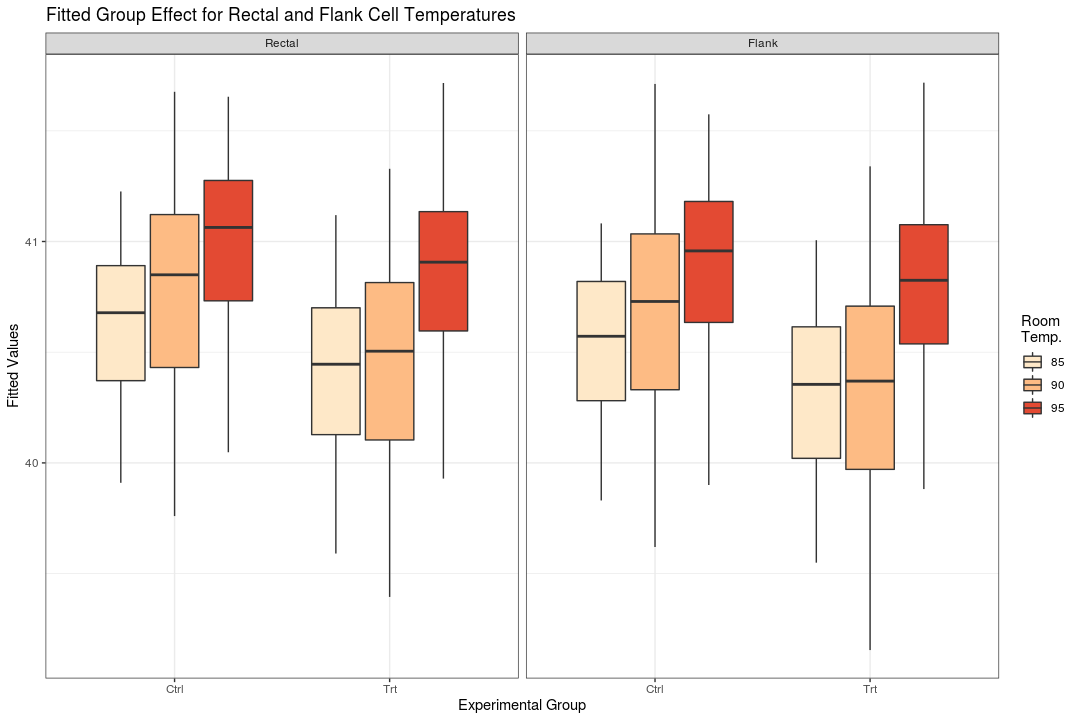
\includegraphics[width = 0.85\textwidth]{images/grp_fit_plot.png}
	\caption{Box plot of fitted group effect for rectal and flank temperature.}
\end{figure}

\begin{figure}[!htbp]
	\centering
		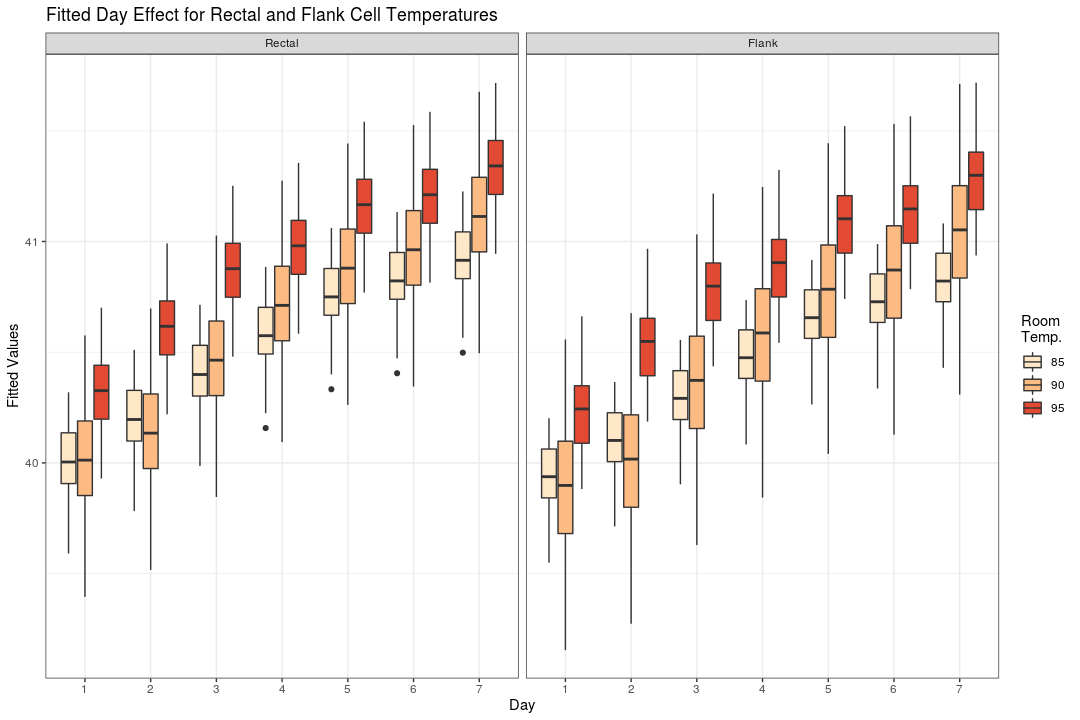
\includegraphics[width = 0.85\textwidth]{images/day_effect_plot.png}
	\caption{Box plot of fitted day effect for rectal and flank temperature.}
\end{figure}

\begin{figure}[!htbp]
	\centering
		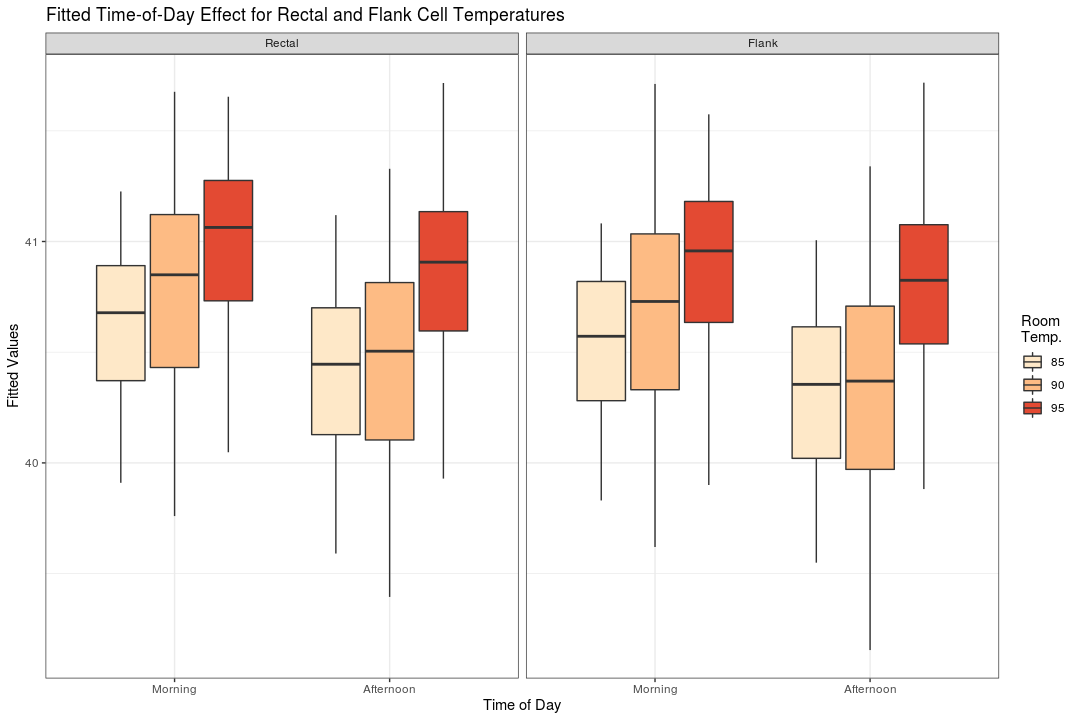
\includegraphics[width = 0.85\textwidth]{images/tod_effect_plot.png}
	\caption{Box plot of fitted time-of-day effect for rectal and flank temperatures.}
\end{figure}

\clearpage

\subsection{R Output}
\subsubsection{Flank vs. Rectal Investigation}
\begin{lstlisting}[basicstyle = \footnotesize \ttfamily]
> rand_fr_mdl <- lme(body_temp_diff_adj~day, random =~1|id
+                        , data = chicken_trans_noout)
> summary(rand_fr_mdl)
Linear mixed-effects model fit by REML
 Data: chicken_trans_noout 
        AIC       BIC   logLik
  -15048.93 -14987.86 7533.466

Random effects:
 Formula: ~1 | id
        (Intercept) Residual
StdDev:  0.06083652  0.07414

Fixed effects: body_temp_diff_adj ~ day 
                  Value   Std.Error   DF    t-value p-value
(Intercept) -0.10235137 0.006662261 6448 -15.362859  0.0000
day2        -0.00609834 0.003417194 6448  -1.784605  0.0744
day3        -0.01152490 0.003407444 6448  -3.382271  0.0007
day4        -0.01253501 0.003431204 6448  -3.653240  0.0003
day5        -0.00057058 0.003429607 6448  -0.166369  0.8679
day6        -0.00435649 0.003433096 6448  -1.268967  0.2045
day7         0.01256056 0.003423788 6448   3.668615  0.0002
 Correlation: 
     (Intr) day2   day3   day4   day5   day6  
day2 -0.255                                   
day3 -0.256  0.499                            
day4 -0.253  0.496  0.497                     
day5 -0.254  0.496  0.497  0.497              
day6 -0.253  0.496  0.497  0.497  0.497       
day7 -0.254  0.497  0.498  0.497  0.497  0.497

Standardized Within-Group Residuals:
        Min          Q1         Med          Q3         Max 
-3.70057184 -0.71894255  0.08052244  0.55262592  3.46178919 

Number of Observations: 6550
Number of Groups: 96 
> anova(rand_fr_mdl)
            numDF denDF   F-value p-value
(Intercept)     1  6448 282.63462  <.0001
day             6  6448  12.23675  <.0001

\end{lstlisting}

\subsubsection{Cell Body Temperature Analysis}
\begin{lstlisting}[basicstyle = \footnotesize \ttfamily]
> #fitting random-effect models
> chicken_air_mdls <- rep(list(vector("list", 2)), 3)
> for(i in 1:3){
+   
+   loop_temp <- c("85", "90", "95")[i]
+   
+   for(j in 1:2){
+     
+     loop_loc <- c("R", "F")[j]
+     loop_loc_full <- c("Rectal", "Flank")[j]   
+     loop_dat <- filter(chicken_agg, room_temp == i-1, loc == j-1)
+     
+     chicken_air_mdl <- lme(body_temp_T~rep+day+group+time_of_day,
+                          random = ~1|id, 
+                          data = loop_dat)   
+     
+     #printing model summaries
+     cat(paste("\n#############################", 
+                 "\nSUMMARY FOR", loop_temp, "DEGREE", 
+                 toupper(loop_loc_full), "RANDOM-EFFECTS MODEL", 
+                 "\n#############################\n", sep = " "))
+     print(summary(chicken_air_mdl))
+     cat(paste("\n#############################", 
+                 "\nANOVA FOR", loop_temp, "DEGREE", 
+                 toupper(loop_loc_full), "RANDOM-EFFECTS MODEL", 
+                 "\n#############################\n", sep = " "))
+     print(anova(chicken_air_mdl))
+     
+     #assigning model to variable of the form chicken_air_mdl_TEMP_LOC
+     #to be accessed outside of loop
+     nam <- paste(c("chicken_air_mdl", loop_temp, loop_loc), collapse = "_")
+     assign(nam, chicken_air_mdl)
+     
+     #storing fits for later
+     chicken_air_mdls[[i]][[j]] <- chicken_air_mdl
+     
+   }
+   
+ }

############################# 
SUMMARY FOR 85 DEGREE RECTAL RANDOM-EFFECTS MODEL 
#############################
Linear mixed-effects model fit by REML
 Data: loop_dat 
       AIC     BIC    logLik
  272.0456 320.811 -124.0228

Random effects:
 Formula: ~1 | id
        (Intercept)  Residual
StdDev:   0.1528331 0.2913598

Fixed effects: body_temp_T ~ rep + day + group + time_of_day 
                Value  Std.Error  DF  t-value p-value
(Intercept)  40.09693 0.06393850 401 627.1171  0.0000
rep2         -0.04626 0.06085745  29  -0.7601  0.4533
day2          0.19199 0.05150562 401   3.7275  0.0002
day3          0.39535 0.05150562 401   7.6758  0.0000
day4          0.56682 0.05200745 401  10.8988  0.0000
day5          0.74217 0.05200745 401  14.2704  0.0000
day6          0.81444 0.05200745 401  15.6601  0.0000
day7          0.90745 0.05200745 401  17.4484  0.0000
group1       -0.21824 0.06085745  29  -3.5861  0.0012
time_of_day1  0.07576 0.02778006 401   2.7272  0.0067
 Correlation: 
             (Intr) rep2   day2   day3   day4   day5   day6   day7   group1
rep2         -0.473                                                        
day2         -0.403  0.000                                                 
day3         -0.403  0.000  0.500                                          
day4         -0.399 -0.007  0.495  0.495                                   
day5         -0.399 -0.007  0.495  0.495  0.494                            
day6         -0.399 -0.007  0.495  0.495  0.494  0.494                     
day7         -0.399 -0.007  0.495  0.495  0.494  0.494  0.494              
group1       -0.473 -0.007  0.000  0.000  0.007  0.007  0.007  0.007       
time_of_day1 -0.217  0.000  0.000  0.000  0.000  0.000  0.000  0.000  0.000

Standardized Within-Group Residuals:
        Min          Q1         Med          Q3         Max 
-4.03665377 -0.52579775  0.04255726  0.55509586  3.13975921 

Number of Observations: 440
Number of Groups: 32 

############################# 
ANOVA FOR 85 DEGREE RECTAL RANDOM-EFFECTS MODEL 
#############################
            numDF denDF   F-value p-value
(Intercept)     1   401 1773039.3  <.0001
rep             1    29       0.3  0.6053
day             6   401      84.1  <.0001
group           1    29      12.9  0.0012
time_of_day     1   401       7.4  0.0067

############################# 
SUMMARY FOR 85 DEGREE FLANK RANDOM-EFFECTS MODEL 
#############################
Linear mixed-effects model fit by REML
 Data: loop_dat 
       AIC      BIC    logLik
  270.1271 318.8925 -123.0635

Random effects:
 Formula: ~1 | id
        (Intercept)  Residual
StdDev:   0.1378869 0.2923181

Fixed effects: body_temp_T ~ rep + day + group + time_of_day 
                Value  Std.Error  DF  t-value p-value
(Intercept)  40.04758 0.06077238 401 658.9768  0.0000
rep2         -0.07007 0.05625592  29  -1.2455  0.2229
day2          0.16383 0.05167502 401   3.1705  0.0016
day3          0.35395 0.05167502 401   6.8496  0.0000
day4          0.53392 0.05217174 401  10.2340  0.0000
day5          0.71477 0.05217174 401  13.7003  0.0000
day6          0.78668 0.05217174 401  15.0786  0.0000
day7          0.88021 0.05217174 401  16.8714  0.0000
group1       -0.22058 0.05625592  29  -3.9211  0.0005
time_of_day1  0.07083 0.02787144 401   2.5413  0.0114
 Correlation: 
             (Intr) rep2   day2   day3   day4   day5   day6   day7   group1
rep2         -0.459                                                        
day2         -0.425  0.000                                                 
day3         -0.425  0.000  0.500                                          
day4         -0.421 -0.008  0.495  0.495                                   
day5         -0.421 -0.008  0.495  0.495  0.494                            
day6         -0.421 -0.008  0.495  0.495  0.494  0.494                     
day7         -0.421 -0.008  0.495  0.495  0.494  0.494  0.494              
group1       -0.459 -0.008  0.000  0.000  0.008  0.008  0.008  0.008       
time_of_day1 -0.229  0.000  0.000  0.000  0.000  0.000  0.000  0.000  0.000

Standardized Within-Group Residuals:
        Min          Q1         Med          Q3         Max 
-4.00748870 -0.51808545  0.06425577  0.59284093  3.28658607 

Number of Observations: 440
Number of Groups: 32 

############################# 
ANOVA FOR 85 DEGREE FLANK RANDOM-EFFECTS MODEL 
#############################
            numDF denDF   F-value p-value
(Intercept)     1   401 2065745.8  <.0001
rep             1    29       1.0  0.3231
day             6   401      80.6  <.0001
group           1    29      15.4  0.0005
time_of_day     1   401       6.5  0.0114

############################# 
SUMMARY FOR 90 DEGREE RECTAL RANDOM-EFFECTS MODEL 
#############################
Linear mixed-effects model fit by REML
 Data: loop_dat 
      AIC      BIC  logLik
  181.378 230.3646 -78.689

Random effects:
 Formula: ~1 | id
        (Intercept)  Residual
StdDev:   0.1511067 0.2601687

Fixed effects: body_temp_T ~ rep + day + group + time_of_day 
                Value  Std.Error  DF  t-value p-value
(Intercept)  40.16635 0.06042766 409 664.7014  0.0000
rep2         -0.18481 0.05880908  29  -3.1426  0.0038
day2          0.12202 0.04599176 409   2.6530  0.0083
day3          0.45152 0.04599176 409   9.8174  0.0000
day4          0.69916 0.04599176 409  15.2018  0.0000
day5          0.86720 0.04599176 409  18.8556  0.0000
day6          0.95040 0.04599176 409  20.6646  0.0000
day7          1.10074 0.04599176 409  23.9333  0.0000
group1       -0.32356 0.05880908  29  -5.5018  0.0000
time_of_day1  0.22394 0.02458363 409   9.1094  0.0000
 Correlation: 
             (Intr) rep2   day2   day3   day4   day5   day6   day7   group1
rep2         -0.487                                                        
day2         -0.381  0.000                                                 
day3         -0.381  0.000  0.500                                          
day4         -0.381  0.000  0.500  0.500                                   
day5         -0.381  0.000  0.500  0.500  0.500                            
day6         -0.381  0.000  0.500  0.500  0.500  0.500                     
day7         -0.381  0.000  0.500  0.500  0.500  0.500  0.500              
group1       -0.487  0.000  0.000  0.000  0.000  0.000  0.000  0.000       
time_of_day1 -0.203  0.000  0.000  0.000  0.000  0.000  0.000  0.000  0.000

Standardized Within-Group Residuals:
         Min           Q1          Med           Q3          Max 
-2.623641948 -0.608194198 -0.008351489  0.620005682  3.306210370 

Number of Observations: 448
Number of Groups: 32 

############################# 
ANOVA FOR 90 DEGREE RECTAL RANDOM-EFFECTS MODEL 
#############################
            numDF denDF   F-value p-value
(Intercept)     1   409 1908587.5  <.0001
rep             1    29       9.9  0.0038
day             6   409     167.9  <.0001
group           1    29      30.3  <.0001
time_of_day     1   409      83.0  <.0001

############################# 
SUMMARY FOR 90 DEGREE FLANK RANDOM-EFFECTS MODEL 
#############################
Linear mixed-effects model fit by REML
 Data: loop_dat 
       AIC      BIC    logLik
  203.6225 252.6091 -89.81124

Random effects:
 Formula: ~1 | id
        (Intercept)  Residual
StdDev:   0.1948965 0.2632088

Fixed effects: body_temp_T ~ rep + day + group + time_of_day 
                Value  Std.Error  DF  t-value p-value
(Intercept)  40.07089 0.07146653 409 560.6945  0.0000
rep2         -0.23096 0.07325738  29  -3.1527  0.0037
day2          0.11908 0.04652917 409   2.5593  0.0108
day3          0.47460 0.04652917 409  10.2000  0.0000
day4          0.68882 0.04652917 409  14.8041  0.0000
day5          0.88633 0.04652917 409  19.0490  0.0000
day6          0.97309 0.04652917 409  20.9136  0.0000
day7          1.15439 0.04652917 409  24.8101  0.0000
group1       -0.34827 0.07325738  29  -4.7540  0.0001
time_of_day1  0.22641 0.02487089 409   9.1035  0.0000
 Correlation: 
             (Intr) rep2   day2   day3   day4   day5   day6   day7   group1
rep2         -0.513                                                        
day2         -0.326  0.000                                                 
day3         -0.326  0.000  0.500                                          
day4         -0.326  0.000  0.500  0.500                                   
day5         -0.326  0.000  0.500  0.500  0.500                            
day6         -0.326  0.000  0.500  0.500  0.500  0.500                     
day7         -0.326  0.000  0.500  0.500  0.500  0.500  0.500              
group1       -0.513  0.000  0.000  0.000  0.000  0.000  0.000  0.000       
time_of_day1 -0.174  0.000  0.000  0.000  0.000  0.000  0.000  0.000  0.000

Standardized Within-Group Residuals:
        Min          Q1         Med          Q3         Max 
-2.59600533 -0.63699049 -0.03296797  0.62595822  3.35590712 

Number of Observations: 448
Number of Groups: 32 

############################# 
ANOVA FOR 90 DEGREE FLANK RANDOM-EFFECTS MODEL 
#############################
            numDF denDF   F-value p-value
(Intercept)     1   409 1223049.6  <.0001
rep             1    29       9.9  0.0037
day             6   409     175.8  <.0001
group           1    29      22.6  0.0001
time_of_day     1   409      82.9  <.0001

############################# 
SUMMARY FOR 95 DEGREE RECTAL RANDOM-EFFECTS MODEL 
#############################
Linear mixed-effects model fit by REML
 Data: loop_dat 
      AIC      BIC   logLik
  80.1506 129.1372 -28.0753

Random effects:
 Formula: ~1 | id
        (Intercept)  Residual
StdDev:   0.1566346 0.2297004

Fixed effects: body_temp_T ~ rep + day + group + time_of_day 
                Value  Std.Error  DF  t-value p-value
(Intercept)  40.35463 0.05897313 409 684.2885  0.0000
rep2         -0.06908 0.05948019  29  -1.1614  0.2550
day2          0.29058 0.04060568 409   7.1561  0.0000
day3          0.55088 0.04060568 409  13.5666  0.0000
day4          0.65437 0.04060568 409  16.1151  0.0000
day5          0.84022 0.04060568 409  20.6923  0.0000
day6          0.88502 0.04060568 409  21.7954  0.0000
day7          1.01527 0.04060568 409  25.0032  0.0000
group1       -0.13009 0.05948019  29  -2.1872  0.0369
time_of_day1  0.13333 0.02170465 409   6.1429  0.0000
 Correlation: 
             (Intr) rep2   day2   day3   day4   day5   day6   day7   group1
rep2         -0.504                                                        
day2         -0.344  0.000                                                 
day3         -0.344  0.000  0.500                                          
day4         -0.344  0.000  0.500  0.500                                   
day5         -0.344  0.000  0.500  0.500  0.500                            
day6         -0.344  0.000  0.500  0.500  0.500  0.500                     
day7         -0.344  0.000  0.500  0.500  0.500  0.500  0.500              
group1       -0.504  0.000  0.000  0.000  0.000  0.000  0.000  0.000       
time_of_day1 -0.184  0.000  0.000  0.000  0.000  0.000  0.000  0.000  0.000

Standardized Within-Group Residuals:
        Min          Q1         Med          Q3         Max 
-2.73615630 -0.61334179  0.01640568  0.63552756  6.08156992 

Number of Observations: 448
Number of Groups: 32 

############################# 
ANOVA FOR 95 DEGREE RECTAL RANDOM-EFFECTS MODEL 
#############################
            numDF denDF   F-value p-value
(Intercept)     1   409 1893795.6  <.0001
rep             1    29       1.3  0.2550
day             6   409     156.1  <.0001
group           1    29       4.8  0.0369
time_of_day     1   409      37.7  <.0001

############################# 
SUMMARY FOR 95 DEGREE FLANK RANDOM-EFFECTS MODEL 
#############################
Linear mixed-effects model fit by REML
 Data: loop_dat 
       AIC      BIC    logLik
  75.59928 124.5859 -25.79964

Random effects:
 Formula: ~1 | id
        (Intercept)  Residual
StdDev:   0.1749549 0.2268782

Fixed effects: body_temp_T ~ rep + day + group + time_of_day 
                Value  Std.Error  DF  t-value p-value
(Intercept)  40.24514 0.06339229 409 634.8586  0.0000
rep2         -0.07872 0.06546557  29  -1.2024  0.2389
day2          0.30481 0.04010678 409   7.6000  0.0000
day3          0.55470 0.04010678 409  13.8305  0.0000
day4          0.66089 0.04010678 409  16.4782  0.0000
day5          0.85899 0.04010678 409  21.4175  0.0000
day6          0.90345 0.04010678 409  22.5260  0.0000
day7          1.05541 0.04010678 409  26.3151  0.0000
group1       -0.10488 0.06546557  29  -1.6020  0.1200
time_of_day1  0.13900 0.02143798 409   6.4836  0.0000
 Correlation: 
             (Intr) rep2   day2   day3   day4   day5   day6   day7   group1
rep2         -0.516                                                        
day2         -0.316  0.000                                                 
day3         -0.316  0.000  0.500                                          
day4         -0.316  0.000  0.500  0.500                                   
day5         -0.316  0.000  0.500  0.500  0.500                            
day6         -0.316  0.000  0.500  0.500  0.500  0.500                     
day7         -0.316  0.000  0.500  0.500  0.500  0.500  0.500              
group1       -0.516  0.000  0.000  0.000  0.000  0.000  0.000  0.000       
time_of_day1 -0.169  0.000  0.000  0.000  0.000  0.000  0.000  0.000  0.000

Standardized Within-Group Residuals:
        Min          Q1         Med          Q3         Max 
-2.88027941 -0.57580420  0.02175375  0.60170797  6.28327356 

Number of Observations: 448
Number of Groups: 32 

############################# 
ANOVA FOR 95 DEGREE FLANK RANDOM-EFFECTS MODEL 
#############################
            numDF denDF   F-value p-value
(Intercept)     1   409 1556900.1  <.0001
rep             1    29       1.4  0.2389
day             6   409     169.2  <.0001
group           1    29       2.6  0.1200
time_of_day     1   409      42.0  <.0001


\end{lstlisting}

\subsection{R Code}
\begin{lstlisting}[basicstyle = \footnotesize \ttfamily]
######################
## Import Libraries ##
######################

library(readxl)
library(tidyverse)
library(lubridate)
library(nlme)
library(grid)
library(gridExtra)
library(ggpmisc)

####################
## Importing Data ##
####################

#importing original data; set to correct working directory
chicken_orig <- read_excel("./Air movement temperature data.xlsx", 
                           sheet = "Temperature data")  

#############################
## Variable Transformation ##
#############################

#this is the 13,360-observation data-set for flank-rectal investigation
chicken_trans <-
  chicken_orig %>% 
  
  #renaming variables
  select(day = `Day of age`, time_of_day = `date-time`, 
         body_temp = Temperature, set = Set, 
         loc = `location R = rectal, W = wing`,
         sensor =`Sensor number`, room_temp = `Room temperature (F)`, 
         trial = Trial, rep = Rep, parent_flock = `Parent flock age`,
         group = Group, period = `Period ( P=pen; T=treatment period)`,
         air_velocity = `Air velocity (ft/min)`
  ) %>%
  
  #recoding, creating chick id variable
  mutate(time_of_day = if_else(hour(time_of_day) < 12, 'AM', 'PM'),
         id = paste(paste(sensor, rep, sep = ""), 
                    room_temp, sep = "")) %>% 
  
  #creating factor variables
  mutate_at(c("day", "time_of_day", "set", "loc", 
              "sensor", "room_temp", "trial", "rep", 
              "parent_flock", "group", "period", 
              "air_velocity"), as_factor) %>%
  
  #placing flank and rectal temperatures on same line
  pivot_wider(names_from = loc, values_from = body_temp, 
              names_prefix = "body_temp_") %>%
  
  #creating flank - rectal difference (adj is rounded to 0.1)
  mutate(body_temp_diff = body_temp_W - body_temp_R,
         body_temp_R_adj = round(body_temp_R, 1),
         body_temp_W_adj = round(body_temp_W, 1)) %>%  
  mutate(body_temp_diff_adj = round(body_temp_W_adj 
                                    - body_temp_R_adj, 1)) %>%
  
  #factor version of body temp diff
  mutate(body_temp_diff_fac = factor(body_temp_diff_adj))

#this is the 2,672-observation data for modeling cell body temperature
chicken_agg <- 
  chicken_trans %>%
  
  #dropping unneeded variables
  select(-c(body_temp_diff, body_temp_diff_adj, body_temp_diff_fac,
            body_temp_R_adj, body_temp_W_adj,
            trial, air_velocity, sensor)) %>%
  
  #aggregating data
  group_by(rep, day, time_of_day, room_temp, group, period, id) %>%
  summarize_at(c("body_temp_W", "body_temp_R"), mean) %>%
  pivot_longer(starts_with("body_temp"), 
               names_to = "loc", 
               values_to = "body_temp") %>%
  pivot_wider(names_from = period, 
              values_from = body_temp, 
              names_prefix = "body_temp_") %>%
  ungroup %>%
  
  #placing flank and rectal measurements on different lines
  mutate_at("loc", as_factor) %>%
  
  #recoding variables
  mutate(time_of_day = fct_recode(time_of_day, "0" = "AM", "1" = "PM"),
         room_temp = fct_recode(room_temp, "0" = "85", "1" = "90", "2" = "95"),
         group = fct_recode(group, "0" = "Ctrl", "1" = "Trt"),
         loc = fct_recode(loc, "0" = "body_temp_R", "1" = "body_temp_W")) %>%
  mutate(body_temp_diff = body_temp_T - body_temp_P,
         group = fct_relevel(group, c("0", "1")),
         loc = fct_relevel(loc, c("0", "1")),
         num_day = as.numeric(day)
  )

#################################
##### Flank-Rectal Modeling #####
#################################

#model from naively regressing flank vs rectal temperature
simple_fr_mdl <- lm(body_temp_W_adj~body_temp_R_adj, data = chicken_trans)
summary(simple_fr_mdl)

#identifying outliers
count(chicken_trans, body_temp_diff_fac)
#removing outliers
chicken_trans_noout <- filter(chicken_trans, 
                              body_temp_diff_adj <= 0.1, 
                              body_temp_diff_adj >= -0.3)

#random-effects model
rand_fr_mdl <- lme(body_temp_diff_adj~day, random =~1|id
                       , data = chicken_trans_noout)
summary(rand_fr_mdl)
anova(rand_fr_mdl)

##############################
##### Flank-Rectal Plots #####
##############################

#scatterplot for flank and rectal temp
ggplot(chicken_trans, aes(x = body_temp_R_adj, y = body_temp_W_adj)) +
  geom_point() +
  geom_smooth(method = "lm", se = F, col = "red") +
  stat_poly_eq(formula = y~x, 
               aes(label = paste(..eq.label.., ..rr.label.., sep = "~~~")), 
               parse = TRUE) +
  xlab("Rectal Body Temp") + ylab("Flank Body Temp") +
  ggtitle("Flank vs Rectal Body Temp") +
  theme(text=element_text(size=21)) +
  scale_x_continuous(breaks = round(seq(36.5, 42.5, by = 0.5), 1)) +
  theme_bw()

#plot of residuals from simple model
simple_fr_preds <- tibble(fit = predict(simple_fr_mdl),
                          res = residuals(simple_fr_mdl))
ggplot(simple_fr_preds, aes(x = fit, y = res)) +
  geom_point() +
  geom_hline(yintercept = mean(simple_fr_preds$res),
             color = "red", linetype = "dashed") +
  xlab("Fitted Values") + ylab("Residuals") +
  ggtitle("Residuals vs Fitted Values for Flank~Rectal Regression") +
  theme(text=element_text(size=21)) +
  theme_bw()  # Add theme for cleaner look

#histogram of flank-rectal temp
ggplot(chicken_trans, aes(x = body_temp_diff_fac)) +
  geom_bar() +
  xlab("Flank - Rectal Temp") +
  ggtitle("Histogram of Flank-Rectal Temp Difference") +
  theme_bw()

#predicted difference values vs rectal temperatures
chicken_trans_noout$fit <- predict(rand_fr_mdl)
ggplot(chicken_trans_noout, aes(x = body_temp_R_adj, y = fit)) +
  geom_point() +
  geom_hline(yintercept = mean(chicken_trans_noout$fit), color = "red", linetype = "dashed") +
  xlab("Rectal Temperature") + ylab("Fitted Flank-Rectal Difference") +
  ggtitle("Fitted Values for Flank-Rectal Difference from Mixed-Effects Model") +
  theme(text=element_text(size=21)) +
  theme_bw()

######################################
### Cell Body Temperature Modeling ###
######################################

#fixed effects
for(i in 1:2){
  
  loop_loc <- c("R", "F")[i]
  loop_loc_full <- c("Rectal", "Flank")[i]
  
  for(j in 1:4){
  
    #1-way ANOVA
    var1 <- c("group", "time_of_day", "room_temp", "day")[j]
    form1 <- paste0("body_temp_T ~ ", var1)
    one_way_mdl <- lm(as.formula(form1), data = filter(chicken_agg, loc == i-1))
    
    #printing anova table
    cat(paste("\n#############################", 
                "\nANOVA FOR 1-WAY", toupper(var1), 
                toupper(loop_loc_full), "MODEL", 
                "\n#############################\n", sep = " "))
    print(anova(one_way_mdl))   
    
    #assigning 1-way model to variables of the form 
    #VAR1_mdl_LOC for access outside of loop   
    nam <- paste(c(var1, "mdl", loop_loc), collapse = "_")
    assign(nam, one_way_mdl)
    
    for(k in which(1:4 > j)){
      
      #2-way ANOVA
      var2 <- c("group", "time_of_day", "room_temp", "day")[k]
      form2 <- paste0("body_temp_T ~ ", var1, "*", var2)
      two_way_mdl <- lm(as.formula(form2), data = filter(chicken_agg, loc == i-1))     

      #printing anova table
      cat(paste("\n#############################", 
                  "\nANOVA FOR 2-WAY", toupper(var1), "*", 
                  toupper(var2), toupper(loop_loc_full), "MODEL", 
                  "\n#############################\n", sep = " "))
      print(anova(two_way_mdl))   
      
      #assigning 2-way model to variables of the form 
      #VAR1_VAR2_mdl_LOC for access outside of loop
      nam <- paste(c(var1, var2, "mdl", loop_loc), collapse = "_")
      assign(nam, two_way_mdl)
      
    }
  
  } 
}

#fitting random-effect models
chicken_air_mdls <- rep(list(vector("list", 2)), 3)
for(i in 1:3){
  
  loop_temp <- c("85", "90", "95")[i]
  
  for(j in 1:2){
    
    loop_loc <- c("R", "F")[j]
    loop_loc_full <- c("Rectal", "Flank")[j]   
    loop_dat <- filter(chicken_agg, room_temp == i-1, loc == j-1)
    
    chicken_air_mdl <- lme(body_temp_T~rep+day+group+time_of_day,
                         random = ~1|id, 
                         data = loop_dat)   
    
    #printing model summaries
    cat(paste("\n#############################", 
                "\nSUMMARY FOR", loop_temp, "DEGREE", 
                toupper(loop_loc_full), "RANDOM-EFFECTS MODEL", 
                "\n#############################\n", sep = " "))
    print(summary(chicken_air_mdl))
    cat(paste("\n#############################", 
                "\nANOVA FOR", loop_temp, "DEGREE", 
                toupper(loop_loc_full), "RANDOM-EFFECTS MODEL", 
                "\n#############################\n", sep = " "))
    print(anova(chicken_air_mdl))
    
    #assigning model to variable of the form chicken_air_mdl_TEMP_LOC
    #to be accessed outside of loop
    nam <- paste(c("chicken_air_mdl", loop_temp, loop_loc), collapse = "_")
    assign(nam, chicken_air_mdl)
    
    #storing fits for later
    chicken_air_mdls[[i]][[j]] <- chicken_air_mdl
    
  }
  
}

#######################################
##### Cell Body Temperature Plots #####
#######################################

#EDA: plotting body temperature for explanatory variables
#function to get legend
get_legend<-function(myggplot){
  tmp <- ggplot_gtable(ggplot_build(myggplot))
  leg <- which(sapply(tmp$grobs, function(x) x$name) == "guide-box")
  legend <- tmp$grobs[[leg]]
  return(legend)
}

#plot to obtain universal legend
legend_plot <- ggplot(chicken_agg, aes(x = group, y = body_temp_T, fill = group)) +
  geom_boxplot(show.legend = T) +
  scale_fill_brewer(type = "qual", direction = -1, 
                    name = "Exp. \nGroup", labels = c("Ctrl", "Trt")) +
  scale_x_discrete(labels = c("0" = "Ctrl", "1" = "Trt")) +
  ggtitle("Experimental Group") + 
  theme_bw() +
  theme(axis.title.x = element_blank(), axis.title.y = element_blank(),
        panel.border=element_rect(fill=NA)) +
  facet_wrap(~loc, labeller = labeller(loc = c(`0` = "Rectal", `1` = "Flank")))

legend <- get_legend(legend_plot)

#cell temp by group
plot1 <- ggplot(chicken_agg, aes(x = group, y = body_temp_T, fill = group)) +
  geom_boxplot(show.legend = F) +
  scale_fill_brewer(type = "qual", direction = -1,
                    name = "Exp. \nGroup", labels = c("Ctrl", "Trt")) +
  scale_x_discrete(labels = c("0" = "Ctrl", "1" = "Trt")) +
  ggtitle("Experimental Group") + 
  theme_bw() +
  theme(axis.title.x = element_blank(), axis.title.y = element_blank(),
        panel.border=element_rect(fill=NA)) +
  facet_wrap(~loc, labeller = labeller(loc = c(`0` = "Rectal", `1` = "Flank")))

#cell temp by time-of-day
plot2 <- ggplot(chicken_agg, aes(x = time_of_day, y = body_temp_T, fill = group)) +
  geom_boxplot(show.legend = F) +
  scale_fill_brewer(type = "qual", direction = -1,
                    labels = c("0" = "Ctrl", "1" = "Trt")) +
  scale_x_discrete(labels = c("0" = "Morning", "1" = "Afternoon")) +
  ggtitle("Time of Day") + 
  theme_bw() +
  theme(axis.title.x = element_blank(), axis.title.y = element_blank(),
        panel.border=element_rect(fill=NA)) +
  facet_wrap(~loc, labeller = labeller(loc = c(`0` = "Rectal", `1` = "Flank")))

#cell temp by room temp
plot3 <- ggplot(chicken_agg, aes(x = room_temp, y = body_temp_T, fill = group)) +
  geom_boxplot(show.legend = F) +
  scale_fill_brewer(type = "qual", direction = -1, 
                    labels = c("0" = "Ctrl", "1" = "Trt")) +
  scale_x_discrete(labels = c("0" = "85", "1" = "90", "2" = "95")) +
  ggtitle("Room Temperature") + 
  theme_bw() +
  theme(axis.title.x = element_blank(), axis.title.y = element_blank(),
        panel.border=element_rect(fill=NA)) +
  facet_wrap(~loc, labeller = labeller(loc = c(`0` = "Rectal", `1` = "Flank")))
  
#cell temp by day
plot4 <- ggplot(chicken_agg, aes(x = day, y = body_temp_T, fill = group)) +
  geom_boxplot(show.legend = F) +
  scale_fill_brewer(type = "qual", direction = -1,
                    labels = c("0" = "Ctrl", "1" = "Trt")) +
  ggtitle("Day") + 
  theme_bw() +
  theme(axis.title.x = element_blank(), axis.title.y = element_blank(),
        panel.border=element_rect(fill=NA)) +
  facet_wrap(~loc, labeller = labeller(loc = c(`0` = "Rectal", `1` = "Flank")))

#cell temp by rep
plot5 <- ggplot(chicken_agg, aes(x = rep, y = body_temp_T, fill = group)) +
  geom_boxplot(show.legend = F) +
  scale_fill_brewer(type = "qual", direction = -1, labels = c("0" = "Ctrl", "1" = "Trt")) +
  ggtitle("Rep") + 
  theme_bw() +
  theme(axis.title.x = element_blank(), axis.title.y = element_blank(),
        panel.border=element_rect(fill=NA)) +
  facet_wrap(~loc, labeller = labeller(loc = c(`0` = "Rectal", `1` = "Flank")))

#arranging plots on common grid
grid.arrange(plot1, plot2, plot3, plot4, plot5, legend,
             top = textGrob("Cell Body Temperature by Factor", gp = gpar(fontsize = 18)),
             left = textGrob("Cell Body Temperature", gp = gpar(fontsize = 18), rot = 90),  
             ncol = 3, nrow = 2)

#analysis: boxplots of fits
#converting fitted values to vector
cell_temp_fits <- chicken_air_mdls %>%
  flatten %>%
  map("fitted") %>%
  map(as_tibble) %>%
  bind_rows %>%
  .$id

#creating dataframe for boxplots
cell_temp_dfs <- lapply(0:2, function(i){
                      lapply(0:1, function(j){
                        return(filter(chicken_agg, room_temp == i, loc == j))
                      })
        }) %>%
  flatten %>%
  bind_rows %>%
  mutate(fit = cell_temp_fits) %>%
  select(loc, room_temp, day, time_of_day, group, fit)

#fitted group effect
ggplot(data = cell_temp_dfs, aes(x = group, y = fit, fill = room_temp)) +
  geom_boxplot() +
  scale_fill_brewer(type = "seq", palette = 8, direction = 1,
                    name = "Room \nTemp.", labels = c("85", "90", "95")) + 
  scale_x_discrete(labels = c("0" = "Ctrl", "1" = "Trt")) + 
  facet_wrap(~loc, labeller = labeller(loc = c(`0` = "Rectal", `1` = "Flank"))) +
  xlab("Experimental Group") + ylab("Fitted Values") +
  ggtitle("Fitted Group Effect for Rectal and Flank Cell Temperatures") +
  theme_bw()

#fitted day effect
ggplot(data = cell_temp_dfs, aes(x = day, y = fit, fill = room_temp)) +
  geom_boxplot() +
  scale_fill_brewer(type = "seq", palette = 8, direction = 1,
                    name = "Room \nTemp.", labels = c("85", "90", "95")) + 
  facet_wrap(~loc, labeller = labeller(loc = c(`0` = "Rectal", `1` = "Flank"))) +
  xlab("Day") + ylab("Fitted Values") +
  ggtitle("Fitted Day Effect for Rectal and Flank Cell Temperatures") +
  theme_bw()

#fitted time-of-day effect
ggplot(data = cell_temp_dfs, aes(x = group, y = fit, fill = room_temp)) +
  geom_boxplot() +
  scale_fill_brewer(type = "seq", palette = 8, direction = 1,
                    name = "Room \nTemp.", labels = c("85", "90", "95")) + 
  scale_x_discrete(labels = c("0" = "Morning", "1" = "Afternoon")) + 
  facet_wrap(~loc, labeller = labeller(loc = c(`0` = "Rectal", `1` = "Flank"))) +
  xlab("Time of Day") + ylab("Fitted Values") +
  ggtitle("Fitted Time-of-Day Effect for Rectal and Flank Cell Temperatures") +
  theme_bw()

\end{lstlisting}

\end{document}

